%% =====================================================================
%% GeoRipple: IEEE conference paper (IEEEtran, conference mode)
%%
%% NOTE TO AUTHORS
%%  - All reported numbers come from the benchmark repo (results/).
%%  - Map figures are in figures/ (generated by
%%    experiments/make_figures.py in the benchmark repo). Upload the
%%    figures/ folder next to this .tex file.
%%  - Fill in author blocks and anonymize if the venue is double-blind.
%% =====================================================================
\documentclass[conference]{IEEEtran}
\IEEEoverridecommandlockouts

\usepackage{cite}
\usepackage{amsmath,amssymb,amsfonts}
\usepackage{algorithm}
\usepackage{algpseudocode}
\usepackage{graphicx}
\usepackage{textcomp}
\usepackage{xcolor}
\usepackage{booktabs}
\usepackage{url}
\usepackage{tikz}
\usetikzlibrary{arrows.meta,positioning,calc}

\newcommand{\tbd}{\textcolor{red}{\textbf{[TBD]}}}
\newcommand{\figplaceholder}[1]{%
  \fbox{\parbox[c][3.6cm][c]{0.92\linewidth}{\centering\small\itshape #1}}}

\def\BibTeX{{\rm B\kern-.05em{\sc i\kern-.025em b}\kern-.08em
    T\kern-.1667em\lower.7ex\hbox{E}\kern-.125emX}}

\begin{document}

\title{GeoRipple: Hazard-Aware Spatio-Topological Disruption Wavefronts
for Resolving Supply-Chain Disruptions with Linked Graph and GIS Views}

\author{
\IEEEauthorblockN{1\textsuperscript{st} Given Name Surname}
\IEEEauthorblockA{\textit{dept. name of organization} \\
\textit{name of organization}\\
City, Country \\
email address or ORCID}
\and
\IEEEauthorblockN{2\textsuperscript{nd} Given Name Surname}
\IEEEauthorblockA{\textit{dept. name of organization} \\
\textit{name of organization}\\
City, Country \\
email address or ORCID}
}

\maketitle

\begin{abstract}
Supply-chain disruptions caused by hurricanes, floods, winter storms, and
wildfires are simultaneously \emph{spatial} events and \emph{network}
events: a hazard strikes a geographic footprint, but its business impact
travels along supplier--distributor--retailer relationships and arrives at
downstream locations days later, after inventory buffers are exhausted.
Existing tools usually treat these two aspects separately. Graph
databases reveal what connects to what; GIS tools reveal what lies inside
the hazard zone. We present \emph{GeoRipple}, a framework and visual
analytics system that unifies them. GeoRipple makes three moves. First,
it treats every transportation lane in the supply-chain graph as a
geometric object (a routed polyline), so that hazards can sever edges and
not only nodes. Second, it propagates hazard-induced capacity loss through
the graph in time, using per-node inventory buffers, to compute a
\emph{disruption wavefront}: the predicted time at which each downstream
location runs out of stock, rendered as an animated front on the map.
Third, it resolves the disruption by generating candidate recovery lanes
through spatial search, validating them with hazard-avoiding road routes,
and selecting a mitigation plan with a time-expanded mixed-integer flow
model. We describe the formulation, a Spatio-Topological Criticality
Index (STCI) for ranking exposed facilities, an implementation on Neo4j,
Snowflake geospatial functions, a routing engine with polygon exclusion,
and linked Leaflet/Cytoscape.js views. On a synthetic benchmark of 15
network--hazard runs, GeoRipple predicts hazard-attributable stockouts with
0.97 precision and a 6.9-day mean timing error, and its plans cut total
unmet demand by 38\% relative to no action, whereas a greedy
nearest-facility heuristic raises total unmet demand at three times the
cost.
\end{abstract}

\begin{IEEEkeywords}
supply-chain resilience, disruption management, knowledge graphs,
geographic information systems, ripple effect, visual analytics,
network flow optimization, hazard-aware routing
\end{IEEEkeywords}

%% ---------------------------------------------------------------------
\section{Introduction}
%% ---------------------------------------------------------------------
When a hurricane makes landfall near a port city, the first question a
supply-chain team asks is geographic: \emph{which of our facilities are
inside the affected area?} The second question is relational:
\emph{who depends on those facilities?} The third question, which matters
most, is temporal and prescriptive: \emph{when will customers actually
feel the shortage, and what can we do before that happens?}

Answering these questions today typically requires three disconnected
artifacts. A GIS layer shows the hazard footprint and facility
locations. A graph or ERP view shows supplier and distribution
relationships. A spreadsheet or planning tool holds inventory positions.
Analysts reconcile the three by hand, under time pressure, during the
very window in which action is still possible.

Two observations motivate this work. First, the literature on
supply-chain disruption has established that impact propagates through
the network with delay, a phenomenon known as the \emph{ripple effect}
\cite{ivanov2017ripple,dolgui2018ripple}, and that the delay is governed
largely by buffers, captured by metrics such as time-to-survive (TTS) and
time-to-recover (TTR) \cite{simchilevi2014,simchilevi2015}. Second,
disruptions frequently sever \emph{transportation lanes} rather than
facilities. A distribution center outside a flood zone is still cut off
if the only interstate corridor feeding it runs through that zone.
Graph-only analyses that remove affected nodes miss this entirely, and
map-only analyses that highlight affected points cannot express it
either.

We present GeoRipple, which couples a supply-chain knowledge graph with
geospatial hazard data to predict and resolve disruptions. Its
contributions are:
\begin{itemize}
  \item \textbf{Lane-geometry enrichment.} Every edge of the supply-chain
  graph is materialized as a routed road (or mode-specific) polyline, so
  that hazard exposure is computed for edges as well as nodes
  (Section~\ref{sec:lanes}).
  \item \textbf{Disruption wavefront.} A time-stepped propagation model
  that converts hazard-induced capacity loss into a predicted
  stockout time for every node, visualized as a moving front on the map
  and as a synchronized coloring of the graph (Section~\ref{sec:wave}).
  \item \textbf{Spatio-Topological Criticality Index (STCI).} A ranking
  that combines hazard exposure, downstream demand-at-risk, and
  structural centrality, so that planners act first on facilities that
  are both exposed and structurally important (Section~\ref{sec:stci}).
  \item \textbf{Hazard-aware resolution.} A mitigation planner that
  generates candidate recovery lanes by spatial search, validates each
  against a routing engine with the hazard polygon excluded, and selects
  a plan with a time-expanded mixed-integer flow model
  (Section~\ref{sec:resolve}).
  \item \textbf{Linked graph--map visual analytics} implemented over
  Neo4j, Snowflake, and Leaflet/Cytoscape.js, plus an evaluation
  protocol grounded in historical hazard footprints
  (Sections~\ref{sec:system}--\ref{sec:eval}).
\end{itemize}

The novel element is the closed loop from a geographic hazard feed,
through topological and temporal propagation, back to a
geographically validated repair plan, with both the problem and the
solution shown on the same linked map and graph.

%% ---------------------------------------------------------------------
\section{Related Work}
%% ---------------------------------------------------------------------
\subsection{Supply-Chain Disruption and the Ripple Effect}
Operations research has studied disruption extensively; Snyder
\textit{et al.}~\cite{snyder2016} survey models for facility failure,
sourcing, and inventory under disruption risk. Ivanov and colleagues
formalize the ripple effect, in which local disruptions cascade through
multi-echelon networks \cite{ivanov2017ripple,dolgui2018ripple}, and
review recovery strategies \cite{ivanov2017review}. Simchi-Levi
\textit{et al.} introduce TTR and TTS as practical, buffer-aware metrics
for identifying high-impact nodes that conventional spend-based risk
scoring misses \cite{simchilevi2014,simchilevi2015}. Sheffi and Rice
\cite{sheffi2005} and Tang \cite{tang2006} frame resilience in terms of
redundancy and flexibility. These works model time and topology but
generally treat geography as an input label rather than as geometry that
hazards intersect.

\subsection{Network-Structural Resilience}
Kim \textit{et al.}~\cite{kim2015} show that the structure of a supply
network, not only node-level attributes, determines whether a single
failure disrupts the network. Centrality measures such as betweenness
\cite{freeman1977,brandes2001} are commonly used to flag structurally
critical nodes. Such measures are hazard-agnostic: a node with high
betweenness is not urgent if no hazard is near it.

\subsection{Geovisualization of Networks}
Flow maps \cite{phan2005,jenny2017} and edge bundling
\cite{holten2006,holten2009} address the clutter that arises when
relational data is drawn over geography. These techniques focus on
legibility of static flows. They do not model how a disruption moves
through the flows over time.

\subsection{Integrated Graph and GIS Platforms}
Commercial platforms increasingly combine graph storage with map views;
for example, Esri's ArcGIS Knowledge links a graph store to ArcGIS maps
\cite{esriknowledge}. Graph databases such as Neo4j support point types
and distance predicates \cite{neo4j}, and cloud warehouses such as
Snowflake provide native \texttt{GEOGRAPHY} types with intersection
predicates \cite{snowflakegeo}. These platforms provide the
\emph{capability} to co-locate graph and geometry but do not prescribe a
method for disruption propagation or resolution.

\subsection{Gap}
To our knowledge, prior work does not combine (i) hazard intersection
with \emph{edges} as geometric lanes, (ii) buffer-aware temporal
propagation to a per-node stockout time, and (iii) hazard-constrained
spatial generation of repair lanes, inside a single linked graph--map
analytic loop. GeoRipple targets this combination.

%% ---------------------------------------------------------------------
\section{Problem Formulation}
%% ---------------------------------------------------------------------
Let $G=(V,E)$ be a directed supply-chain graph. Nodes $V$ are partitioned
into suppliers $V_S$, distribution centers $V_D$, and demand points
(e.g., dealerships or stores) $V_R$. Each node $v$ has a location
$p_v\in\mathbb{R}^2$ (longitude, latitude), a throughput capacity
$\kappa_v$, an on-hand inventory $I_v(0)$, and, for $v\in V_R$, a demand
rate $d_v(t)$. Each edge $e=(u,v)\in E$ has a capacity $\kappa_e$, a
transit time $\tau_e$, a unit cost $c_e$, and a \emph{lane geometry}
$\gamma_e$, a polyline from $p_u$ to $p_v$ along the transport network.

\textbf{Hazard.} A hazard is a time-indexed family of polygons with
severity, $\mathcal{H}=\{(H_k(t), s_k)\}$, where $H_k(t)\subset
\mathbb{R}^2$ and $s_k\in[0,1]$ is the fraction of capacity lost inside
region $k$. Forecast products (e.g., hurricane track cones, flood
inundation extents, wildfire perimeters) supply $\mathcal{H}$ directly or
as an ensemble of $M$ scenarios $\{\mathcal{H}^{(m)}\}_{m=1}^{M}$ with
probabilities $\pi_m$.

\textbf{Objective.} Given $G$, $\mathcal{H}$, and horizon $T$, (a)
predict for every node the stockout time
$\sigma_v\in\{0,\dots,T\}\cup\{\infty\}$ and the demand-at-risk
$\mathrm{DaR}_v$; (b) rank nodes by urgency; and (c) choose a set of
mitigation actions that minimizes unmet demand plus mitigation cost,
subject to the hazard.

%% ---------------------------------------------------------------------
\section{The GeoRipple Framework}
%% ---------------------------------------------------------------------
Fig.~\ref{fig:pipeline} summarizes the pipeline.

\begin{figure}[t]
\centering
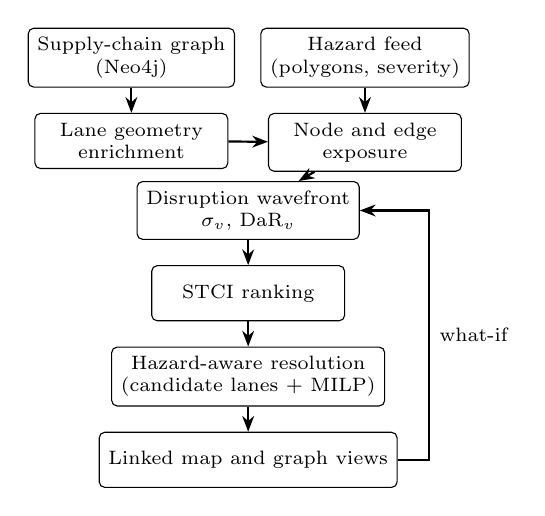
\begin{tikzpicture}[
  node distance=3.2mm,
  box/.style={draw, rounded corners=2pt, align=center,
              font=\scriptsize, minimum width=2.45cm, minimum height=7mm},
  arr/.style={-{Stealth[length=2mm]}, thick}]
  \node[box] (g)  {Supply-chain graph\\(Neo4j)};
  \node[box, right=of g] (h) {Hazard feed\\(polygons, severity)};
  \node[box, below=of g] (l) {Lane geometry\\enrichment};
  \node[box, below=of h] (x) {Node and edge\\exposure};
  \node[box, below=5mm of $(l)!0.5!(x)$] (w) {Disruption wavefront\\$\sigma_v$, DaR$_v$};
  \node[box, below=of w] (s) {STCI ranking};
  \node[box, below=of s] (r) {Hazard-aware resolution\\(candidate lanes + MILP)};
  \node[box, below=of r] (v) {Linked map and graph views};
  \draw[arr] (g) -- (l);
  \draw[arr] (h) -- (x);
  \draw[arr] (l) -- (x);
  \draw[arr] (x) -- (w);
  \draw[arr] (w) -- (s);
  \draw[arr] (s) -- (r);
  \draw[arr] (r) -- (v);
  \draw[arr] (v.east) -- ++(4mm,0) |- node[pos=0.25, right, font=\scriptsize]{what-if} (w.east);
\end{tikzpicture}
\caption{GeoRipple pipeline. The analyst's what-if edits in the linked
views (e.g., marking a facility offline or adjusting severity) feed back
into wavefront recomputation.}
\label{fig:pipeline}
\end{figure}

\subsection{Lane-Geometry Enrichment}\label{sec:lanes}
Node locations are resolved from native geometry when available, and
otherwise from address or postal-code centroids. For each edge $e=(u,v)$
we request a mode-appropriate route between $p_u$ and $p_v$ from a
routing engine and store the resulting polyline $\gamma_e$ together with
its duration, which initializes $\tau_e$. Lanes are stored as
\texttt{GEOGRAPHY} values in the warehouse, keyed by the graph edge
identifier, so that spatial predicates can be evaluated in bulk. Where a
lane is not road-based (rail, air), $\gamma_e$ is a rail-network route or
a great-circle segment, respectively. Enrichment is performed once and
refreshed only when an edge is added or its mode changes.

\subsection{Hazard Exposure of Nodes and Edges}
For a node, exposure at time $t$ is the largest severity of any hazard
region containing it:
\begin{equation}
x_v(t) = \max_{k:\,p_v\in H_k(t)} s_k, \qquad x_v(t)=0 \text{ if none.}
\end{equation}
For an edge, a single blocked segment can close the lane, so exposure is
driven by the most severe region the lane crosses, weighted by how much
of the lane lies inside it:
\begin{equation}
x_e(t) = \max_{k}\; s_k \cdot
\min\!\left(1,\; \frac{|\gamma_e\cap H_k(t)|}{\ell_{\min}}\right),
\end{equation}
where $|\cdot|$ is length and $\ell_{\min}$ is a short threshold length
(e.g., 1\,km) above which any crossing is treated as fully exposed. This
reflects that a road closure anywhere on a lane blocks the whole lane.
Effective capacities are then
$\tilde\kappa_v(t)=\kappa_v\,(1-x_v(t))$ and
$\tilde\kappa_e(t)=\kappa_e\,(1-x_e(t))$. Both exposures are computed
with a single batched \texttt{ST\_INTERSECTS}/\texttt{ST\_INTERSECTION}
query over the stored lane and node geometries.

\subsection{Disruption Wavefront Propagation}\label{sec:wave}
Given degraded capacities, we simulate flow in discrete time steps over
horizon $T$ (Algorithm~\ref{alg:wave}). Each node forwards material
along its outgoing edges according to its baseline allocation shares
$\alpha_e$ (the fraction of $v$'s outflow normally sent on $e$), subject to
effective capacity, and shipments arrive after $\tau_e$ steps. Demand
points consume at rate $d_v(t)$. A node's stockout time $\sigma_v$ is
the first step at which its inventory is exhausted and inflow is
insufficient to cover demand. All lanes into a node share its
hazard-degraded receiving capacity $\kappa^{\mathrm{in}}_v(1-x_v(t))$;
shipments are scaled down proportionally when this is exceeded, so that
opening parallel lanes into a flooded area cannot bypass the hazard.

The \emph{wavefront} at time $t$ is the set
$W(t)=\{v:\sigma_v\le t\}$. Its geographic rendering is the moving
boundary of $W(t)$ on the map. Because inventory buffers delay
propagation, a demand point far from the hazard may enter $W(t)$ before
a nearby one with more stock. This is exactly the counterintuitive
behavior that a map-only or graph-only view hides. Demand-at-risk
accumulates unmet demand over the horizon:
\begin{equation}
\mathrm{DaR}_v = \sum_{t=0}^{T} \max\bigl(0,\; d_v(t)-q_v(t)\bigr),
\end{equation}
where $q_v(t)$ is the quantity actually served. For upstream nodes,
$\mathrm{DaR}^{\downarrow}_v$ denotes the total DaR of demand points
whose baseline supply passes through $v$. Under a hazard ensemble we
report expectations $\mathbb{E}[\sigma_v]$ and $\mathbb{E}[\mathrm{DaR}_v]$
over scenarios weighted by $\pi_m$, and render the probability
$\Pr[\sigma_v\le t]$ as the wavefront's opacity. Each simulation costs
$O(T\,|E|)$; scenarios are independent and run in parallel.

\begin{algorithm}[t]
\caption{Disruption wavefront propagation}
\label{alg:wave}
\begin{algorithmic}[1]
\Require $G$, capacities $\tilde\kappa_v(t),\tilde\kappa_e(t)$,
  shares $\alpha_e$, inventories $I_v(0)$, demand $d_v(t)$, horizon $T$
\Ensure stockout times $\sigma_v$, served quantities $q_v(t)$
\State $\sigma_v\gets\infty$ for all $v$; pipeline queue $Q\gets\emptyset$
\For{$t=0$ \textbf{to} $T$}
  \ForAll{$v\in V$}
    \State $a_v\gets$ arrivals in $Q$ due at $t$ for $v$
    \State $I_v\gets I_v + a_v$
    \If{$v\in V_S$} $I_v\gets I_v + \tilde\kappa_v(t)$ \EndIf
    \If{$v\in V_R$}
      \State $q_v(t)\gets\min(I_v,\,d_v(t))$;\; $I_v\gets I_v-q_v(t)$
      \If{$q_v(t)<d_v(t)$ \textbf{and} $\sigma_v=\infty$}
        $\sigma_v\gets t$ \EndIf
    \Else
      \State $o_v\gets\min(I_v,\,\tilde\kappa_v(t))$
      \ForAll{$e=(v,w)\in E$}
        \State $f_e\gets\min(\alpha_e\,o_v,\ \tilde\kappa_e(t))$
        \State push $(w,\,f_e)$ into $Q$ due at $t+\tau_e$;\;
               $I_v\gets I_v-f_e$
      \EndFor
      \If{$o_v<$ baseline outflow of $v$ \textbf{and} $\sigma_v=\infty$}
        $\sigma_v\gets t$ \EndIf
    \EndIf
  \EndFor
\EndFor
\end{algorithmic}
\end{algorithm}

\subsection{Spatio-Topological Criticality Index}\label{sec:stci}
Planners need a short list of where to act. Exposure alone ignores
structure; centrality alone ignores the hazard. We define
\begin{equation}
\mathrm{STCI}_v = \hat{x}_v \cdot \widehat{\mathrm{DaR}}^{\downarrow}_v
\cdot \bigl(1 + \lambda\,\hat{B}_v\bigr),
\label{eq:stci}
\end{equation}
where $\hat{x}_v$ is the expected peak exposure of $v$ \emph{or of any of
its inbound lanes}, $\widehat{\mathrm{DaR}}^{\downarrow}_v$ is normalized
expected downstream demand-at-risk, $\hat{B}_v$ is normalized
flow-weighted betweenness \cite{brandes2001}, and $\lambda\ge0$ controls
the structural bonus. The product form encodes a deliberate property:
a facility with no hazard exposure receives zero criticality for the
current event, however central it is, while a lightly exposed facility
that funnels large downstream demand ranks highly. Including inbound-lane
exposure in $\hat{x}_v$ allows a facility outside the hazard zone to be
flagged when its feeding corridors are cut.

\subsection{Hazard-Aware Resolution}\label{sec:resolve}
Resolution proceeds in two stages: spatial generation of candidate
actions, then optimization.

\textbf{Candidate generation.} For each node $v$ with
$\mathbb{E}[\sigma_v]\le T$, we generate candidate recovery lanes of four
kinds: (i) \emph{reroute}, an alternative existing path in $G$ whose
lanes have low exposure; (ii) \emph{lateral transshipment}, a new lane
from a peer distribution center; (iii) \emph{alternate sourcing}, a new
lane from a qualified supplier not currently serving $v$; and (iv)
\emph{expedite}, a mode change on an existing lane that shortens
$\tau_e$. For kinds (ii) and (iii), we run a spatial $k$-nearest-neighbor
query over unexposed nodes of the permissible type within radius $R$,
filtered by graph constraints (e.g., the candidate supplier must be
linked to a compatible part via the knowledge graph). Each surviving pair
is sent to a routing engine with the buffered hazard polygons supplied as
\emph{exclusion areas}. Pairs whose origin lies inside the hazard, or
whose route duration exceeds a maximum $\tau_{\max}$, are discarded. When
only the destination lies inside the hazard, the lane must enter it
regardless; it is kept with its forecast exposure attached, so the
optimizer can still use it before onset (e.g., to pre-position stock).
The result is a candidate edge set $E_c$ whose geometries avoid
\emph{crossing} the forecast hazard. To keep planning interactive,
candidates are generated only for dealers downstream of the top-$K$
facilities by STCI and for those facilities themselves.

\textbf{Optimization.} On the time-expanded network over $E\cup E_c$, let
$f_e^t\ge0$ be flow departing on $e$ at step $t$, $I_v^t\ge0$ inventory,
$u_v^t\ge0$ unmet demand at $v\in V_R$, and $y_e\in\{0,1\}$ the
activation of candidate lane $e\in E_c$ with fixed cost $F_e$. We solve
\begin{align}
\min\ & \sum_{t}\sum_{e} c_e f_e^t + \sum_{e\in E_c} F_e\,y_e
       + \sum_{t}\sum_{v\in V_R} \rho_v\,u_v^t \label{eq:obj}\\
\text{s.t.}\ & I_v^{t} = I_v^{t-1} + \!\!\sum_{e=(w,v)}\! f_e^{t-\tau_e}
   - \!\!\sum_{e=(v,w)}\! f_e^{t} \nonumber\\
& \qquad\quad + b_v^t - d_v^t + u_v^t \quad \forall v,\ \forall t \label{eq:bal}\\
& f_e^t \le \tilde\kappa_e(t) \quad \forall e\in E,\ \forall t \label{eq:cap}\\
& f_e^t \le \kappa_e\, y_e \quad \forall e\in E_c,\ \forall t \label{eq:act}\\
& \textstyle\sum_{e=(v,w)} f_e^t \le \tilde\kappa_v(t) \quad \forall v,\ \forall t
  \label{eq:nodecap}\\
& \textstyle\sum_{e=(w,v)} f_e^t \le \kappa^{\mathrm{in}}_v\,(1-x_v(t)) \quad \forall v,\ \forall t
  \label{eq:recvcap}
\end{align}
where $b_v^t=\tilde\kappa_v(t)$ is production for $v\in V_S$ (zero
otherwise), $d_v^t=0$ and $u_v^t=0$ for $v\notin V_R$, and $\rho_v$ is a
shortage penalty that may encode customer priority. Constraint
\eqref{eq:cap} enforces hazard-degraded capacity on existing lanes, and
\eqref{eq:act} opens candidate lanes only if activated. Under an
ensemble, we solve a two-stage stochastic variant in which $y_e$ is
chosen here-and-now and flows are scenario-dependent. For interactive
speed, our prototype instead solves a single risk-averse problem in which
each exposure is set to its upper quartile across forecast members;
averaging exposures would understate a hazard that is severe in some
members and absent in others. Plans are executed additively: each
existing lane ships the larger of its baseline and planned quantity, and
activated recovery lanes ship their planned flows.

The MILP is small because candidate generation prunes $E_c$ spatially
and temporally. The planner returns actions ranked by marginal DaR
reduction per unit cost, which the interface displays alongside the
wavefront they are predicted to push back.

%% ---------------------------------------------------------------------
\section{System Implementation}\label{sec:system}
%% ---------------------------------------------------------------------
\textbf{Data tier.} The supply-chain knowledge graph resides in Neo4j
\cite{neo4j}, with typed nodes (\texttt{Supplier},
\texttt{DistributionCenter}, \texttt{Dealership}, \texttt{Part},
\texttt{Disruption}) and relationships (\texttt{SUPPLIES},
\texttt{DISTRIBUTES\_TO}, \texttt{COMPATIBLE\_WITH}). Lane and hazard
geometries reside in Snowflake as \texttt{GEOGRAPHY} columns, where
exposure is computed with \texttt{ST\_INTERSECTS} and
\texttt{ST\_INTERSECTION} \cite{snowflakegeo}. Edge identifiers join the
two stores. Hazard polygons are ingested from public forecast feeds as
GeoJSON and versioned by issue time, so that each analysis is
reproducible against the forecast that was available when it ran.

\textbf{Routing.} Lane enrichment uses OSRM \cite{osrm}. Hazard-avoiding
routing for candidate lanes uses a self-hosted routing engine that
accepts exclusion polygons, such as Valhalla \cite{valhalla} or
GraphHopper custom models \cite{graphhopper}. Self-hosting avoids the
usage limits of public demo servers and keeps facility addresses
internal.

\textbf{Analytics tier.} Wavefront simulation (Algorithm~\ref{alg:wave})
is vectorized over scenarios. The MILP is solved with an open-source
solver such as HiGHS \cite{highs}. Betweenness is computed with the
Neo4j Graph Data Science library and cached between hazard updates, since
it depends only on topology and flows.

\textbf{Presentation tier.} A React front end renders a Leaflet map
\cite{leaflet} and a Cytoscape.js graph \cite{franz2016} as linked views.
Selecting a node in either view selects it in the other. The map shows
hazard polygons, exposed lanes drawn as dashed red polylines, and demand
points colored by $\mathbb{E}[\sigma_v]$ on a sequential scale. A time
slider animates $W(t)$ as the wavefront advances. Recommended recovery
lanes appear as solid arcs; toggling one re-solves the wavefront and
visibly pushes back the front. The graph view uses the same color scale,
so that an analyst can see where the shortage appears on the map and why
it arises in the graph. Edge rendering is gated by zoom level and by
selection to maintain legibility at national scale.

\textbf{Explanations.} An optional natural-language panel summarizes the
top STCI facilities and the chosen plan. Graph data passed to the
language model is filtered server-side by a per-type property allow-list,
so that commercially sensitive attributes never leave the analytics tier.

Figs.~\ref{fig:wavefront} and~\ref{fig:resolution} show the two map views
for one run of the benchmark in Section~\ref{sec:eval}.

\begin{figure}[t]
\centering
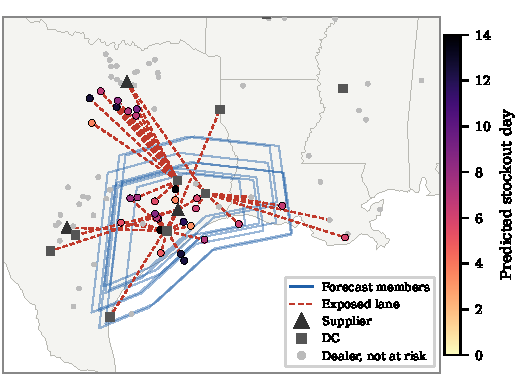
\includegraphics[width=\linewidth]{figures/fig_wavefront.pdf}
\caption{Wavefront view for one benchmark run (Gulf hurricane flood,
seed 0), rendered with the map view's encodings. Blue outlines are the
eight forecast members; dashed red lines are the 45 lanes whose mean
peak exposure across members is at least 0.5. The 29 dealers predicted to stock out are shaded by
predicted stockout day; gray dealers are not at risk.}
\label{fig:wavefront}
\end{figure}

\begin{figure}[t]
\centering
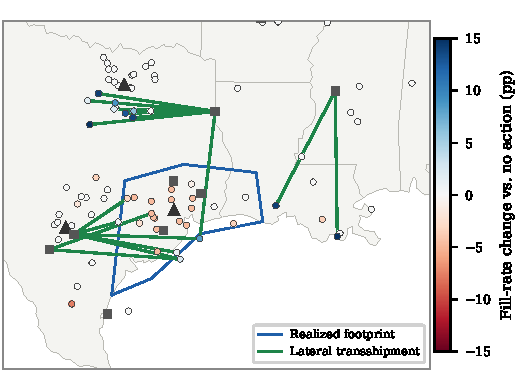
\includegraphics[width=\linewidth]{figures/fig_resolution.pdf}
\caption{Resolution view for the same run. Green lines are the 16
lateral-transshipment lanes activated by the MILP; dealers are shaded by
their change in fill rate versus no action under the realized footprint
(blue outline). The plan cut unmet demand from 1{,}234 to 651 units at a
cost of \$24.2k; 29 dealers improved and one was slightly worse off.}
\label{fig:resolution}
\end{figure}

%% ---------------------------------------------------------------------
\section{Evaluation}\label{sec:eval}
%% ---------------------------------------------------------------------
\subsection{Benchmark}
We evaluate on synthetic three-echelon networks with 20 suppliers, 60
distribution centers, and 600 dealerships, placed with Gaussian jitter
around approximate coordinates of 59 U.S.\ metropolitan areas, dealers in
proportion to metro population. Each dealer is served by its nearest
distribution center, and each distribution center by its two nearest
suppliers. Dealer demand is lognormal (median 10 units/day) and
inventories are lognormal with a median of five days of supply. Lanes
are straight segments scaled by a road factor of 1.25, with transit time
at 700\,km/day. Hazard-avoiding candidate routes are computed with a
visibility graph over the buffered forecast footprint, a stand-in for a
routing engine with exclusion polygons. The horizon is $T=28$ days.

We use three stylized hazard footprints, hand-drawn to resemble event
types that disrupt U.S.\ freight: a Gulf Coast hurricane flood (severity
0.9, days 2--10), a statewide winter storm (severity 0.6, days 2--8), and
a Mississippi River corridor flood (severity 1.0, days 3--14). They are
not reconstructions of specific historical events. GeoRipple sees only a
forecast ensemble of $M=8$ members, generated by perturbing each
footprint's position, extent, timing, and severity. Ground truth comes
from executing the same network under the unperturbed footprint with
Poisson transit delays (mean 0.3 days per shipment). A stockout counts
as \emph{hazard-attributable} if it occurs, or occurs earlier, than in an
otherwise identical run without the hazard, which separates hazard
impact from ordinary delay noise. We run five network seeds for each
hazard, giving 15 runs.

\subsection{Baselines, Ablations, and Metrics}
We compare against (B1) \emph{topology-only}, which marks every dealer
downstream of a facility inside the forecast footprint as stocking out at
onset; (B2) \emph{node-only spatial}, which is GeoRipple without lane
exposure; and (B3) \emph{greedy nearest-facility} recovery, which gives
every predicted-stranded dealer a straight lane from its nearest
unexposed distribution center, shipping full demand from day 0 without
hazard routing or a candidate budget. Ablations remove inventory buffers
(A1), hazard-aware candidate routing so that candidate lanes are
straight and assumed clear when planning (A2), and the structural term
of \eqref{eq:stci} by setting $\lambda=0$ (A3). All planners use $K=10$,
$k=3$ candidates per target, lateral radius 600\,km, sourcing radius
1{,}500\,km, $\tau_{\max}=4$ days, and a shortage penalty of \$100/unit.
The MILP is solved with HiGHS through SciPy with a 1\% optimality gap;
every instance reached that gap. The benchmark implements lateral transshipment
and alternate sourcing as candidate lanes; shifting flow between existing
lanes, which corresponds to rerouting in this network, happens inside the
MILP. Expediting is not evaluated.

Prediction is scored by precision and recall of the set of dealers with
a hazard-attributable stockout, and by the mean absolute error of
$\sigma_v$ over the union of predicted and actual stockouts, with
non-stockouts set to $T$. Fill rate and TTR$_{95}$ are computed over the
dealers affected under no action. TTR$_{95}$ is the number of days from
onset until their aggregate daily fill rate stays at or above 95\%.
Unmet demand is summed over \emph{all} dealers, so that it also counts
harm to dealers from which stock was diverted. Cost is the fixed plus
transport cost of recovery lanes actually used.

\subsection{Results}
\begin{table}[t]
\caption{Stockout prediction versus realized outcome (mean (s.d.) over 15 runs)}
\label{tab:pred}
\centering
\small\setlength{\tabcolsep}{3pt}
\resizebox{\columnwidth}{!}{%
\begin{tabular}{@{}lccc@{}}
\toprule
Method & Prec.$^{\dagger}$ & Recall & MAE $\sigma_v$ (d)\\
\midrule
B1 Topology-only & 0.42 (0.11) & 0.93 (0.15) & 18.3 (2.2) \\
B2 Node-only spatial & 0.98 (0.06) & 0.57 (0.23) & 8.3 (4.0) \\
A1 No buffers & 0.41 (0.08) & 0.99 (0.03) & 16.4 (2.4) \\
GeoRipple (full) & 0.97 (0.06) & 0.65 (0.26) & 6.9 (4.2) \\
\bottomrule
\end{tabular}}
\vspace{2pt}
\parbox{\linewidth}{\footnotesize $^{\dagger}$Averaged over runs with at least one predicted stockout; bracketed superscript gives that count when fewer than all runs.}
\end{table}

\begin{table}[t]
\caption{Resolution quality under realized hazards (mean (s.d.) over 15 runs)}
\label{tab:resolve}
\centering
\small\setlength{\tabcolsep}{2.5pt}
\resizebox{\columnwidth}{!}{%
\begin{tabular}{@{}lcccc@{}}
\toprule
Method & Fill rate & Unmet (u) & TTR$_{95}$ (d) & Cost (\$k)\\
\midrule
No action & 0.854 (0.091) & 1037 (545) & 20.4 (3.2) & 0.0 (0.0) \\
B3 Greedy nearest & 0.919 (0.056) & 1109 (596) & 18.2 (4.5) & 27.2 (12.2) \\
A2 No hazard routing & 0.910 (0.050) & 648 (281) & 19.6 (3.1) & 9.2 (8.1) \\
A3 $\lambda=0$ & 0.910 (0.049) & 646 (259) & 18.9 (3.1) & 9.1 (8.8) \\
GeoRipple (full) & 0.910 (0.049) & 646 (259) & 18.9 (3.1) & 9.1 (8.8) \\
\bottomrule
\end{tabular}}
\end{table}

\textbf{Prediction.} Table~\ref{tab:pred} shows that methods ignoring time
over-alarm. Topology-only (B1) and the no-buffer ablation (A1) flag
nearly every affected dealer but with precision near 0.4, and they place
stockouts about 16--18 days away from when they actually occur, because
they assume shortage arrives at onset. Modeling inventory buffers cuts
the timing error to 6.9 days while keeping precision at 0.97. Adding lane
exposure raises recall from 0.57 to 0.65 overall. The gain is
concentrated in the river flood, where recall rises from 0.54 to 0.79
because many lanes cross the corridor while their endpoints lie outside
it. For the hurricane and winter storm, lane exposure changed no
predictions. Recall remains low for the winter storm (0.33 for both B2
and GeoRipple): at moderate severity, many realized stockouts arise from
the combination of partial capacity loss and transit delays, which the
deterministic forecast simulation does not reproduce.

\textbf{Resolution.} Table~\ref{tab:resolve} shows that GeoRipple's plans
reduce total unmet demand from 1{,}037 to 646 units (38\%) at a mean cost
of \$9.1k, raising fill rate among affected dealers from 0.854 to 0.910.
The greedy heuristic (B3) achieves a slightly higher affected-dealer fill
rate (0.919) and faster recovery, but it \emph{increases} total unmet
demand to 1{,}109 units at three times the cost. It does so by drawing
inventory from unexposed distribution centers without replenishing them,
shifting shortages onto dealers that the hazard never touched. The
optimizer avoids this because it accounts for every dealer's balance.
Recovery time improves only modestly for all methods, since it is
dominated by hazard duration.

\textbf{Negative results.} Two components had little or no measurable
effect here. Hazard-aware routing (A2) changed total unmet demand by only
two units, because within the 600\,km and four-day limits few candidate
lanes crossed a forecast footprint. The structural term (A3) had no
effect at all: the top-$K$ facility set was identical with $\lambda=0$ in
all 15 runs. In these tree-structured networks, betweenness is nearly
proportional to downstream demand and adds no ranking information.
Evaluating both components needs networks with multi-sourcing, cross
docks, and longer recovery lanes.

\textbf{Latency.} End-to-end planning, from forecast exposures to a
solved plan, took 4.9\,s on average and at most 49\,s on a single CPU
core.

\subsection{User Study Protocol}
To evaluate the linked views, we plan a within-subjects study with
supply-chain analysts under three conditions: graph view only, map view
only, and linked GeoRipple views. Tasks include identifying the first
demand point to stock out, identifying a facility outside the hazard
that is nonetheless cut off, and selecting a recovery plan under a cost
cap. We will measure task accuracy, completion time, NASA-TLX workload,
and System Usability Scale scores, with condition order counterbalanced.

\subsection{Reproducibility}
The benchmark code, including network generation, hazard ensembles,
simulation, candidate generation, the MILP, and the scripts that produce
Tables~\ref{tab:pred} and~\ref{tab:resolve}, is available at
\url{https://github.com/<your-account>/georipple-benchmark}.

%% ---------------------------------------------------------------------
\section{Discussion}
%% ---------------------------------------------------------------------
\textbf{Why lanes matter.} Treating edges as geometry changes which
facilities are flagged. A distribution center outside a flood zone but
fed exclusively through it has zero node exposure and would be ignored by
node-based methods; in GeoRipple its inbound-lane exposure raises its
STCI and its downstream demand points appear in the wavefront.

\textbf{Why time matters.} Maps show where a hazard is; they do not show
when customers will feel it. The wavefront reframes the decision window
per location, so planners can prioritize demand points with the least
slack instead of those closest to the hazard.

\textbf{Why optimize over the whole network.} The greedy baseline shows
that local fixes can be net harmful. Rescuing stranded dealers from the
nearest unaffected facility moved shortages elsewhere and raised total
unmet demand. Recovery decisions need to be made against the whole
network's inventory balance, which the linked graph view makes visible
and the MILP makes explicit. Validating repairs against the hazard
geometry remains important in principle, since a recovery lane can cross
the hazard that caused the disruption, although in our benchmark this
occurred rarely.

\textbf{Limitations.} The evaluation is synthetic: facility locations
are jittered around approximate metro coordinates, lanes are straight
segments rather than road routes, and the hazards are stylized footprints
rather than observed ones. The benchmark networks are trees, which
limits what the structural term and rerouting can contribute. The
propagation model uses fixed allocation shares
and does not capture dynamic reallocation by partners, bullwhip effects,
or demand surges during disasters. Postal-code centroids introduce
location error for nodes lacking precise geometry. Hazard severity is
reduced to a single capacity-loss fraction, while real hazards affect
labor, power, and transport differently. Candidate generation assumes
that alternate suppliers are qualified if the knowledge graph links them
to a compatible part, which may not hold in regulated industries.
Finally, the approach depends on the quality of forecast footprints, and
its value is bounded by forecast skill.

%% ---------------------------------------------------------------------
\section{Conclusion and Future Work}
%% ---------------------------------------------------------------------
GeoRipple treats a supply-chain disruption as a single spatio-temporal
object that starts as a geographic hazard, propagates through the network
with buffer-dependent delay, and is resolved by geographically validated
changes to the network. By materializing lanes as geometry, computing a
disruption wavefront, ranking facilities with a hazard-conditioned
criticality index, and generating hazard-avoiding recovery lanes for a
time-expanded optimization, it connects what analysts see on a map with
what they reason about in a graph. Future work includes learning
allocation shares and severities from historical shipment and outage
data, modeling multi-hazard compound events, extending to international
networks with multimodal routing, evaluating on observed hazard
footprints and road-routed lanes over multi-sourced networks, and
conducting the user study described in Section~\ref{sec:eval}.

\section*{Acknowledgment}
% Add funding sources and acknowledgments here, or remove this section.

%% ---------------------------------------------------------------------
\begin{thebibliography}{00}
\bibitem{ivanov2017ripple} D. Ivanov, ``Simulation-based ripple effect
modelling in the supply chain,'' \textit{Int. J. Production Research},
vol. 55, no. 7, pp. 2083--2101, 2017.

\bibitem{dolgui2018ripple} A. Dolgui, D. Ivanov, and B. Sokolov,
``Ripple effect in the supply chain: an analysis and recent literature,''
\textit{Int. J. Production Research}, vol. 56, no. 1--2, pp. 414--430,
2018.

\bibitem{ivanov2017review} D. Ivanov, A. Dolgui, B. Sokolov, and
M. Ivanova, ``Literature review on disruption recovery in the supply
chain,'' \textit{Int. J. Production Research}, vol. 55, no. 20,
pp. 6158--6174, 2017.

\bibitem{simchilevi2014} D. Simchi-Levi, W. Schmidt, and Y. Wei, ``From
superstorms to factory fires: Managing unpredictable supply-chain
disruptions,'' \textit{Harvard Business Review}, vol. 92, no. 1--2,
pp. 96--101, 2014.

\bibitem{simchilevi2015} D. Simchi-Levi \textit{et al.}, ``Identifying
risks and mitigating disruptions in the automotive supply chain,''
\textit{Interfaces}, vol. 45, no. 5, pp. 375--390, 2015.

\bibitem{snyder2016} L. V. Snyder \textit{et al.}, ``OR/MS models for
supply chain disruptions: A review,'' \textit{IIE Transactions}, vol. 48,
no. 2, pp. 89--109, 2016.

\bibitem{sheffi2005} Y. Sheffi and J. B. Rice Jr., ``A supply chain view
of the resilient enterprise,'' \textit{MIT Sloan Management Review},
vol. 47, no. 1, pp. 41--48, 2005.

\bibitem{tang2006} C. S. Tang, ``Perspectives in supply chain risk
management,'' \textit{Int. J. Production Economics}, vol. 103, no. 2,
pp. 451--488, 2006.

\bibitem{kim2015} Y. Kim, Y.-S. Chen, and K. Linderman, ``Supply network
disruption and resilience: A network structural perspective,''
\textit{J. Operations Management}, vol. 33--34, pp. 43--59, 2015.

\bibitem{freeman1977} L. C. Freeman, ``A set of measures of centrality
based on betweenness,'' \textit{Sociometry}, vol. 40, no. 1, pp. 35--41,
1977.

\bibitem{brandes2001} U. Brandes, ``A faster algorithm for betweenness
centrality,'' \textit{J. Mathematical Sociology}, vol. 25, no. 2,
pp. 163--177, 2001.

\bibitem{phan2005} D. Phan, L. Xiao, R. Yeh, P. Hanrahan, and
T. Winograd, ``Flow map layout,'' in \textit{Proc. IEEE Symp. Information
Visualization (InfoVis)}, 2005, pp. 219--224.

\bibitem{jenny2017} B. Jenny \textit{et al.}, ``Design principles for
origin-destination flow maps,'' \textit{Cartography and Geographic
Information Science}, vol. 45, no. 1, pp. 62--75, 2018.

\bibitem{holten2006} D. Holten, ``Hierarchical edge bundles:
Visualization of adjacency relations in hierarchical data,''
\textit{IEEE Trans. Visualization and Computer Graphics}, vol. 12, no. 5,
pp. 741--748, 2006.

\bibitem{holten2009} D. Holten and J. J. van Wijk, ``Force-directed edge
bundling for graph visualization,'' \textit{Computer Graphics Forum},
vol. 28, no. 3, pp. 983--990, 2009.

\bibitem{esriknowledge} Esri, ``ArcGIS Knowledge,'' [Online]. Available:
\url{https://www.esri.com/en-us/arcgis/products/arcgis-knowledge/overview}

\bibitem{neo4j} Neo4j, Inc., ``Neo4j Graph Database,'' [Online].
Available: \url{https://neo4j.com/}

\bibitem{snowflakegeo} Snowflake Inc., ``Geospatial data types,''
Snowflake Documentation. [Online]. Available:
\url{https://docs.snowflake.com/}

\bibitem{osrm} D. Luxen and C. Vetter, ``Real-time routing with
OpenStreetMap data,'' in \textit{Proc. 19th ACM SIGSPATIAL Int. Conf.
Advances in Geographic Information Systems}, 2011, pp. 513--516.

\bibitem{valhalla} Valhalla Contributors, ``Valhalla: Open source routing
engine for OpenStreetMap,'' [Online]. Available:
\url{https://github.com/valhalla/valhalla}

\bibitem{graphhopper} GraphHopper GmbH, ``GraphHopper routing engine:
Custom models,'' [Online]. Available:
\url{https://github.com/graphhopper/graphhopper}

\bibitem{highs} Q. Huangfu and J. A. J. Hall, ``Parallelizing the dual
revised simplex method,'' \textit{Mathematical Programming Computation},
vol. 10, no. 1, pp. 119--142, 2018.

\bibitem{leaflet} Leaflet, ``Leaflet: a JavaScript library for
interactive maps,'' [Online]. Available: \url{https://leafletjs.com/}

\bibitem{franz2016} M. Franz \textit{et al.}, ``Cytoscape.js: a graph
theory library for visualisation and analysis,''
\textit{Bioinformatics}, vol. 32, no. 2, pp. 309--311, 2016.
\end{thebibliography}

\end{document}
